%Notes by Harsh Mistry 
%Econ 301
%Based on Template From  https://www.cs.cmu.edu/~ggordon/10725-F12/template.tex

\documentclass[twoside]{article}
\setlength{\oddsidemargin}{0.25 in}
\setlength{\evensidemargin}{-0.25 in}
\setlength{\topmargin}{-0.6 in}
\setlength{\textwidth}{6.5 in}
\setlength{\textheight}{8.5 in}
\setlength{\headsep}{0.75 in}
\setlength{\parindent}{0 in}
\setlength{\parskip}{0.1 in}
\usepackage{amsmath,amsfonts,graphicx, color}
\newcounter{lecnum}
\renewcommand{\thepage}{\thelecnum-\arabic{page}}
\renewcommand{\thesection}{\thelecnum.\arabic{section}}
\renewcommand{\theequation}{\thelecnum.\arabic{equation}}
\renewcommand{\thefigure}{\thelecnum.\arabic{figure}}
\renewcommand{\thetable}{\thelecnum.\arabic{table}}
\newcommand{\lecture}[4]{
   \pagestyle{myheadings}
   \thispagestyle{plain}
   \newpage
   \setcounter{lecnum}{#1}
   \setcounter{page}{1}
   
   
%Info Box 
   \begin{center}
   \framebox{
      \vbox{\vspace{2mm}
    \hbox to 6.28in { {\bf Econ 301 - Microeconomic Theory 2
	\hfill Winter 2018} }
       \vspace{4mm}
       \hbox to 6.28in { {\Large \hfill Lecture #1: #2  \hfill} }
       \vspace{2mm}
       \hbox to 6.28in { {\it Lecturer: #3 \hfill Notes By: #4} }
      \vspace{2mm}}
   }
   \end{center}
   
   \markboth{Lecture #1: #2}{Lecture #1: #2}



 
}

\renewcommand{\cite}[1]{[#1]}
\def\beginrefs{\begin{list}%
        {[\arabic{equation}]}{\usecounter{equation}
         \setlength{\leftmargin}{2.0truecm}\setlength{\labelsep}{0.4truecm}%
         \setlength{\labelwidth}{1.6truecm}}}
\def\endrefs{\end{list}}
\def\bibentry#1{\item[\hbox{[#1]}]}

\newcommand{\fig}[3]{
			\vspace{#2}
			\begin{center}
			Figure \thelecnum.#1:~#3
			\end{center}
	}
	
	\graphicspath{ {images/} }

\newtheorem{theorem}{Theorem}[lecnum]
\newtheorem{lemma}[theorem]{Lemma}
\newtheorem{ex}[theorem]{Example}
\newtheorem{proposition}[theorem]{Proposition}
\newtheorem{claim}[theorem]{Claim}
\newtheorem{corollary}[theorem]{Corollary}
\newtheorem{definition}[theorem]{Definition}
\newenvironment{proof}{{\bf Proof:}}{\hfill\rule{2mm}{2mm}}
\newcommand\E{\mathbb{E}}


%Start of Document 
\begin{document}

\lecture{3}{January 10, 2018}{Jean Guillaume Forand}{Harsh Mistry}

\section{Consumer Choice Continued}

\begin{itemize}
\item Given a preference relation \(\succeq\) on \(\mathbb{R}_*^2\), 
\begin{itemize}
\item The \underline{strict preference relation} \(\succ\) on \(\mathbb{R}_*^2\) is defined such that \(x > y \) if an only if \(x \succeq y \) but not \(y \succeq x\)
\item The \underline{indifference relation} \(\sim\) on \(\mathbb{R}^2_*\) is defined such that \(x \sim y \) iff \(x \succeq y \) and \(y \succeq x\)
\item Having as primitives the weak preference relation is equivalent to having as primitives the strict preference and indifference relations
\end{itemize}
\item An arbitrary preference relation need not correspond to preferences we find interesting or reasonable
\begin{ex} Fix pref. rel. \(\succeq\) on \(\mathbb{R}_*^2\) 
\begin{enumerate}
\item Say \(\succeq\) such that not \(x \succeq y \) for all \(x, y \in \mathbb{R}_*^2\)
\begin{itemize}
\item Consumer is \textbf{not} indifferent between all bundles, but incapable  of stating preferences
\end{itemize}
\item Say \(\succeq\) is such that there exists \(x, y, z \in \mathbb{R}_*^2\) with \(x \succ y \succ z\) and \(z \succ x\)
\begin{itemize}
\item Ranking of bundles x and z are inconsistent when, 
\begin{itemize}
\item compared through y, x is best
\item compared directly, z is best
\end{itemize}
\end{itemize} 
\end{enumerate}
\end{ex}
\end{itemize}

\begin{definition}
The preference relation \(\succeq\) on \(\mathbb{R}^2_*\) is 
\begin{enumerate}
\item \underline{Complete} if, for all \(x, y \in \mathbb{R}^2_*\), either \(x \succeq y \) or \(y \succ x\) (or both)
\item \underline{Transitive} if, for all \(x, y, z \in \mathbb{R}_*^2\) such that \(x \succeq y \succeq z\), we have \(x \succeq z\)
\end{enumerate}
\end{definition}

\begin{itemize}
\item These are \underline{rationality assumptions}
\item Completeness assumes that DM has capacity to reflect on his preferences
\item Transitivity 
\begin{itemize}
\item is critical theoretically (without it, optimal choices need not exists)
\item is problematic empirically
\begin{itemize}
\item Say good 1 is beer, good 2 is cigarettes
\[x = (2,0) \hspace{0.5cm} y = (0,0),\hspace{0.5cm} z = (2, 1) \]
\end{itemize}
\end{itemize}
\end{itemize}
\begin{definition} Given a preference relation \(
succeq\) on \(\mathbb{R}_*^2\) and a bundle \(z\), the \underline{indifference curve of \(z\)} is the set of \(\{x \in \mathbb{R}_*^2\ ; x \sim z\}\)
\end{definition}
\begin{itemize}
\item Indifference curves need not be line segments
\begin{ex} Say \(\succeq\) on \(\mathbb{R}^2_*\) such that \(x \succeq y\) for all \(x, y \in \mathbb{R}^2_*\)
\begin{center}
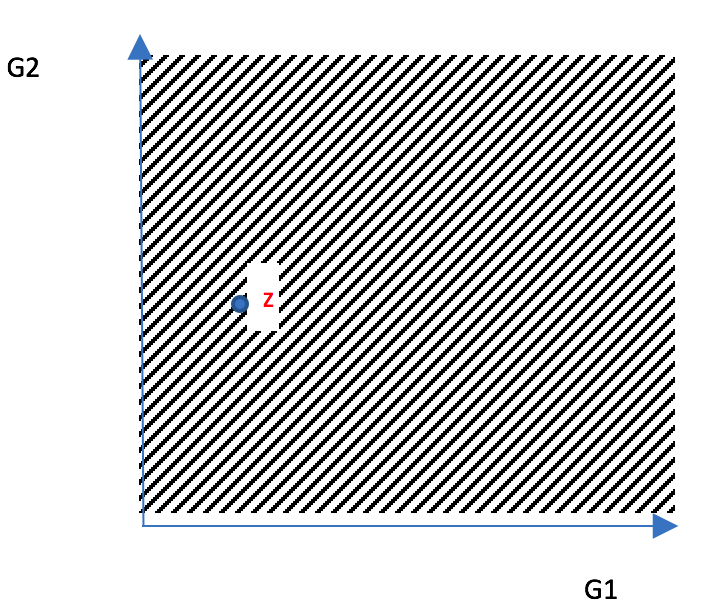
\includegraphics[scale=0.4]{4}
\end{center}
\end{ex}
\item Indifference curves need not be downward sloping.
\begin{ex}
Say \(\succeq\) on \(\mathbb{R}^2_*\) such that there exists bundle \(\hat{x}\) such that \(x \succeq y\) iff \(x\) is lower to \(\hat{x}\) than \(y\) is \begin{itemize}
\item \(\hat{x}\) is the "bliss point"
\end{itemize}
\begin{center}
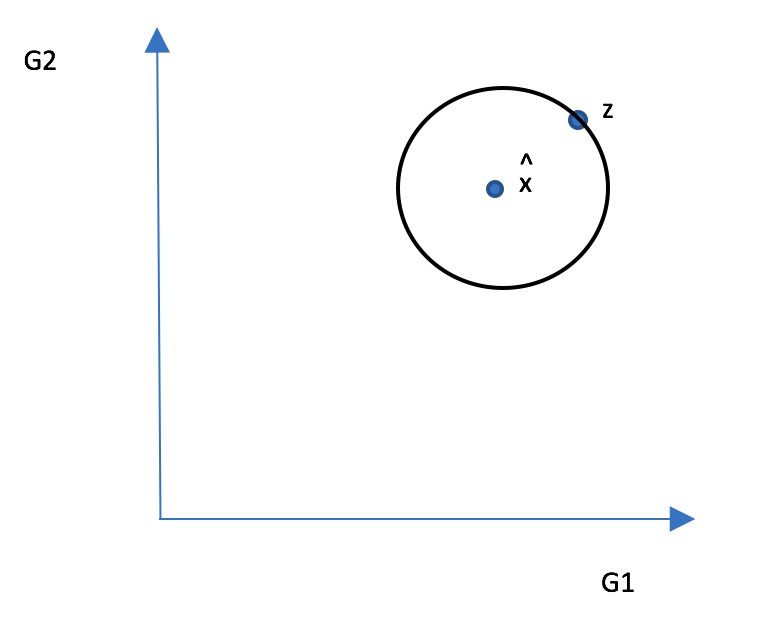
\includegraphics[scale=0.4]{5}
\end{center} \end{ex}
\item Indifference curves need not be smooth or differentiable 
\begin{ex}
Perfect complements, i.e \(\succeq\) on \(\mathbb{R}_*^2\) such that \(x \succeq y \) iff \(min \{ x_1, x_2\} \geq min \{y_1, y_2\}\)
\begin{center}
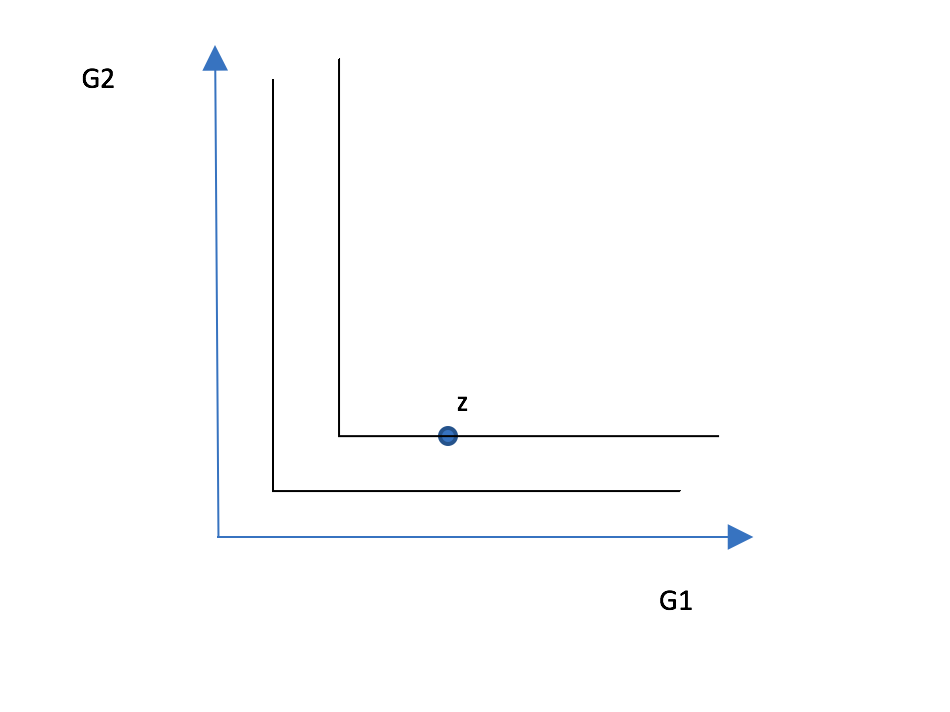
\includegraphics[scale=0.4]{6}
\end{center}
\end{ex}
\end{itemize}

\end{document}





